\documentclass[11pt]{aghdpl}
% \documentclass[en,11pt]{aghdpl}  % praca w języku angielskim

% Lista wszystkich języków stanowiących języki pozycji bibliograficznych użytych w pracy.
% (Zgodnie z zasadami tworzenia bibliografii każda pozycja powinna zostać utworzona zgodnie z zasadami języka, w którym dana publikacja została napisana.)
\usepackage[english,polish]{babel}

% Użyj polskiego łamania wyrazów (zamiast domyślnego angielskiego).
\usepackage{polski}

\usepackage[utf8]{inputenc}

% dodatkowe pakiety

\usepackage{mathtools}
\usepackage{amsfonts}
\usepackage{amsmath}
\usepackage{amsthm}

% --- < bibliografia > ---

\usepackage[
style=numeric,
sorting=none,
%
% Zastosuj styl wpisu bibliograficznego właściwy językowi publikacji.
language=autobib,
autolang=other,
% Zapisuj datę dostępu do strony WWW w formacie RRRR-MM-DD.
urldate=iso8601,
% Nie dodawaj numerów stron, na których występuje cytowanie.
backref=false,
% Podawaj ISBN.
isbn=true,
% Nie podawaj URL-i, o ile nie jest to konieczne.
url=false,
%
% Ustawienia związane z polskimi normami dla bibliografii.
maxbibnames=3,
% Jeżeli używamy BibTeXa:
backend=bibtex
]{biblatex}

\usepackage{csquotes}
% Ponieważ `csquotes` nie posiada polskiego stylu, można skorzystać z mocno zbliżonego stylu chorwackiego.
\DeclareQuoteAlias{croatian}{polish}

\addbibresource{bibliografia.bib}

% Nie wyświetlaj wybranych pól.
%\AtEveryBibitem{\clearfield{note}}


% ------------------------
% --- < listingi > ---

% Użyj czcionki kroju Courier.
\usepackage{courier}

\usepackage{listings}
\lstloadlanguages{TeX}

\lstset{
	literate={ą}{{\k{a}}}1
           {ć}{{\'c}}1
           {ę}{{\k{e}}}1
           {ó}{{\'o}}1
           {ń}{{\'n}}1
           {ł}{{\l{}}}1
           {ś}{{\'s}}1
           {ź}{{\'z}}1
           {ż}{{\.z}}1
           {Ą}{{\k{A}}}1
           {Ć}{{\'C}}1
           {Ę}{{\k{E}}}1
           {Ó}{{\'O}}1
           {Ń}{{\'N}}1
           {Ł}{{\L{}}}1
           {Ś}{{\'S}}1
           {Ź}{{\'Z}}1
           {Ż}{{\.Z}}1,
	basicstyle=\footnotesize\ttfamily,
}

% ------------------------

\AtBeginDocument{
	\renewcommand{\tablename}{Tabela}
	\renewcommand{\figurename}{Rys.}
}

% ------------------------
% --- < tabele > ---

\usepackage{array}
\usepackage{tabularx}
\usepackage{multirow}
\usepackage{booktabs}
\usepackage{makecell}
\usepackage[flushleft]{threeparttable}

% defines the X column to use m (\parbox[c]) instead of p (`parbox[t]`)
\newcolumntype{C}[1]{>{\hsize=#1\hsize\centering\arraybackslash}X}


%---------------------------------------------------------------------------

\author{Marcin Szpyrka}
\shortauthor{M. Szpyrka}

%\titlePL{Przygotowanie bardzo długiej i pasjonującej pracy dyplomowej w~systemie~\LaTeX}
%\titleEN{Preparation of a very long and fascinating bachelor or master thesis in \LaTeX}

\titlePL{Przygotowanie pracy dyplomowej w~systemie~\LaTeX}
\titleEN{Thesis in \LaTeX}


\shorttitlePL{Przygotowanie pracy dyplomowej w~systemie \LaTeX} % skrócona wersja tytułu jeśli jest bardzo długi
\shorttitleEN{Preparation of a long and fascinating thesis in \LaTeX}

\thesistype{Praca dyplomowa magisterska}
%\thesistype{Master of Science Thesis}

\supervisor{prof. dr hab. Marcin Szpyrka}
%\supervisor{Marcin Szpyrka PhD, DSc}

\degreeprogramme{Informatyka}
%\degreeprogramme{Computer Science}

\date{2015}

\department{Katedra Informatyki Stosowanej}
%\department{Department of Applied Computer Science}

\faculty{Wydział Elektrotechniki, Automatyki,\protect\\[-1mm] Informatyki i Inżynierii Biomedycznej}
%\faculty{Faculty of Electrical Engineering, Automatics, Computer Science and Biomedical Engineering}

\acknowledgements{Serdecznie dziękuję \dots tu ciąg dalszych podziękowań np. dla promotora, żony, sąsiada itp.}


\setlength{\cftsecnumwidth}{10mm}

%---------------------------------------------------------------------------
\setcounter{secnumdepth}{4}
\brokenpenalty=10000\relax

\begin{document}

\titlepages

% Ponowne zdefiniowanie stylu `plain`, aby usunąć numer strony z pierwszej strony spisu treści i poszczególnych rozdziałów.
\fancypagestyle{plain}
{
	% Usuń nagłówek i stopkę
	\fancyhf{}
	% Usuń linie.
	\renewcommand{\headrulewidth}{0pt}
	\renewcommand{\footrulewidth}{0pt}
}

\setcounter{tocdepth}{2}
\tableofcontents
\clearpage

\chapter{Nawigacje dla rowerzystów}
\label{cha:nawigacje_dla_rowerzystow}

Nawigacja jako ogólne zagadnienie funkcjonuje w świadomości ludzi już od dłuższego czasu. Wprawdzie jeszcze 20-25 lat temu mało kto wyobrażał sobie jazdę samochodem po nieznanych terenach bez wcześniejszego zaplanowania trasy przy pomocy papierowej mapy, to jednak ostatnia dekada przyniosła w zasadzie całkowite wyparcie takiego stanu rzeczy. Odpowiadają za to właśnie nawigacje, najpierw jako autonomiczne urządzenia, potem jako aplikacje na smartfony (choć te pierwsze nadal funkcjonują na rynku i mają się całkiem dobrze).

\section{Specyfika tematu}
Bardzo duży staż rynkowy nawigacji daje podstawy do stwierdzenia, że wszystko co istotne zostało już w tej materii wymyślone i zaimplementowane. Być może jest to prawda, a być może czeka nas jeszcze niejedna rewolucja (z gatunku raczej tych nie zauważalnych przez przeciętnego użytkownika), co nie zmienia jednak faktu, że fundamenty są i zapewne pozostaną te same. Nawigacje bowiem w dużej mierze opierają swe działanie na poprawności czterech głównych czynników:
\begin{itemize}
\item dokładnych i aktualnych danych o infrastrukturze 
\item zbudowania grafu relacji powyższych danych
\item możliwie jak najbardziej efektywnego i optymalnego algorytmu do wyszukiwania najkrótszej ścieżki w tymże grafie
\item przejrzystej i intuicyjnej wizualizacji wyników
\end{itemize}
I tak jak ostatni punkt, to w dużej mierze kwestia estetyki (choć oczywiście nie tylko), tak pierwsze trzy bardzo mocno wpływają na jakość wskazań. W przypadku konkretnie nawigacji rowerowych największą trudnością jest punkt pierwszy. Prawidłowe dane na temat ścieżek rowerowych, czy też dróg przyjaznych rowerzystom, to towar mocno deficytowy. Jednakże nawet jego posiadanie nie gwarantuje pełni sukcesu, gdyż tematyka infrastruktury rowerowej jest znacznie bardziej złożona aniżeli infrastruktury samochodowej. W tym drugim przypadku działa prosty warunek: jest droga znaczy da się przejechać. Oczywiście należy także uwzględnić chociażby kierunkowość ulic, jednak na tym poziom komplikacji się w zasadzie kończy. Z rowerem sprawa wygląda inaczej, gdyż czasami bardzo trudno jest jednoznacznie określić wszystkie miejsca, przez które da się oraz można przejechać rowerem. Przeszkodą mogą być zwykłe schody, czy też samo-zamykająca się brama, bądź szlaban. Działa to także w drugą stronę: dwie sąsiadujące ze sobą lokalne uliczki mogą nie być połączone w rozumieniu samochodowym, a jednak dzielić je może jedynie pas betonowych donic na kwiaty lub słupki. Przykłady można by mnożyć bez końca, niemożliwym jest uwzględnienie absolutnie każdej realnie możliwej relacji, zwłaszcza w przypadku większej skali, jak obszar całego państwa. W mniejszym zakresie – jak rozpiętość średniej wielkości miasta, jakim jest Kraków – jest to w większym lub mniejszym stopniu wykonalne, choć z pewnością niełatwe i wymagające wielu testów praktycznych wykonanych bezpośrednio w terenie. Podobnym problemem jest kwalifikacja zwykłych dróg, na te przyjazne rowerom oraz te nieprzyjazne. Wprawdzie dylemat ten, w przypadku niniejszej aplikacji, został niejako rozwiązany przez osoby trzecie, gdyż ZIKiT sam dostarcza również dane o preferowanych ulicach do użytku także rowerowego, to jednak nie da się ukryć pewnego drobnego paradoksu z tym związanego. Otóż ulice przyjazne rowerzyście powinny charakteryzować się możliwie jak najniższą prędkością maksymalną zdefiniowaną dla pojazdów mechanicznych oraz relatywnie małym natężeniem ruchu tychże. Takie ulice to zazwyczaj lokalne drogi osiedlowe, których przecież jedynym celem jest doprowadzenie ruchu do większych arterii, a te już przyjazne rowerzyście z pewnością nie są. Oczywiście można mieć nadzieje, że każda większa trasa komunikacyjna będzie posiadać równoległą do siebie ścieżką rowerową, ale niestety w Krakowie na ten moment nie ma to jeszcze miejsca.\newline
Warto się także pochylić nad wspomnianą wcześniej bazą danych ZIKiTu odnoszącą się do dróg przyjaznych rowerzyście. Zostały one zdefiniowane jako tzw. drogi tempo 30, czyli takie na których obowiązuje ograniczenie prędkości do 30 km/h. Bardzo trudno o rzetelny osąd takiego, a nie innego wyboru. Prawdopodobnie wynikało to z chęci stworzenia jak najbardziej kompletnej sieci możliwych dróg.Gdzie konkretnie zdefiniowane zostały strefy z tego typu drogami można zobaczyć na mapie wizualizacji dancyh ZIKiTu (Rys. 3.1.).\newline

\begin{figure}[H]
\centering
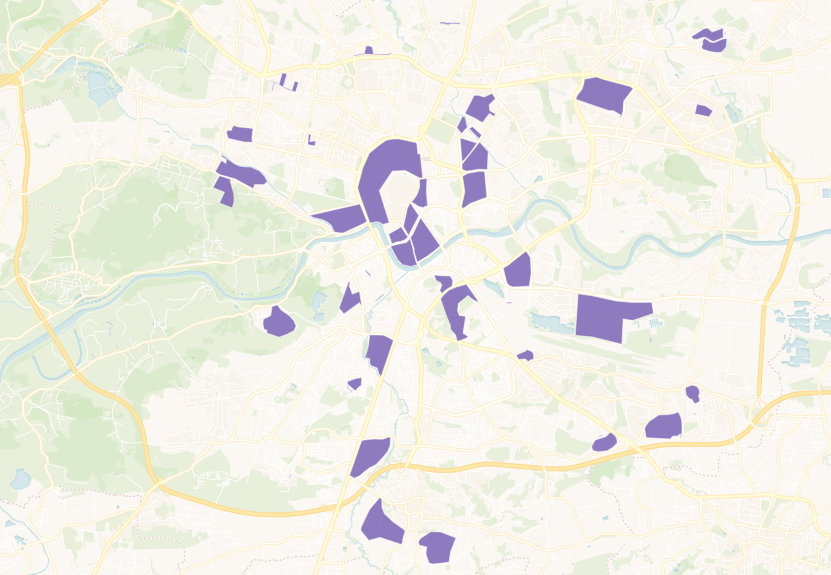
\includegraphics[width=\textwidth]{tempo30}
\caption{Strefy tzw. ulic tempo 30; źródło ZIKiT: \protect\url{https://zikit.carto.com/tables/tempo30krakow/public\#/map} (stan na dzień 6.09.2019).}
\end{figure}

Kwestia poprawnego grafu relacji to także trudny temat. Samo jego zbudowanie to jedno, wielokroć istotniejszą sprawą w kontekście nawigacji rowerowej jest waga danych ścieżek. Chodzi oczywiście o – nierzadką przecież – sytuację, gdy w dane miejsce prowadzą zarówno autonomiczne ścieżki rowerowe (rozdzielone od jezdni), te wyznaczone w torze jezdni samochodowej oraz drogi z kategorii przyjaznych rowerzyście. W jaki sposób odpowiednio dobrać wagi? Co całkowicie zrozumiałe nie mogą być one równoważne, gdyż wtedy dochodziłoby do absurdalnych sytuacji, gdy nawigacja prowadziłaby po samych drogach samochodowych tylko dlatego, że trasa po autonomicznej ścieżce rowerowa byłaby dłuższa, dajmy na to, dosłownie o parę metrów. Wagi te nie mogą być także zbyt zróżnicowane, gdyż wtedy dochodziłoby do sytuacji odwrotnych: nawigacja sugerowałaby wprawdzie trasę po samych autonomicznych ścieżkach rowerowych, ale znacznie dłuższą, niż gdyby skorzystać w paru miejscach ze „skrótu” w postaci drogi lokalnej. Stąd tak ważne jest by autorzy takiej nawigacji dobrze znali obszar ( w tym przypadku miasto Kraków), po którym ma ona prowadzić. Bez praktycznej znajomości topografii, mogłoby być ciężko wykryć pewne błędy w postaci nielogicznych tras.

\section{Istniejące rozwiązania}

Światowy rynek nawigacji rowerowych nie grzeszy obfitością, nie mówiąc już o rozwiązaniach stricte dla terenów Polski. Oczywiście funkcjonują rozwiązania gigantów jak choćby Mapy Google (zarówno wersja webowa jak i na urządzenia mobilne), czy Mapy Apple (wyłącznie na urządzenie mobilne), jednak ich główną domeną jest nawigacja przygotowana dla samochodów, odmiana dla rowerzystów, to raczej dodatek traktowany obecnie nieco po macoszemu i oparty na nie do końca sprawdzonych danych, co wyraźnie widać w ich działaniu. Dlatego też rozwiązania te wpadają w proste pułapki jak na przykład wyznaczanie trasy przez schody bądź pomijanie tzw. kontrapasów rowerowych. Nie ma się jednak temu co dziwić, jeśli weźmiemy pod uwagę ogrom obszaru jaki obejmują niniejsze projekty. Niemałym problemem w ich przypadku jest również mocne opóźnienie aktualizacji w stosunku do rzeczywistych zmian w infrastrukturze. Istnieją oczywiście również profesjonalne urządzenia nazywane „nawigacją rowerową”, jednak są to produkty dość drogie i skierowane raczej do co najmniej średnio-zaawansowanych rowerzystów, a nie do człowieka, który po prostu chce dostać się do pracy przy pomocy rowery. Inną sprawą jest, ze tego typu profesjonalne nawigacje starają się za wszelką cenę unikać zatłoczonych tras i większych miast, siłą rzeczy więc nie nadają się do nawigowania po metropoliach. \newline
Osobnym przypadkiem jest aplikacja Bike Citizens, dostępna zarówno w formie webowej jak i na urządzenia mobilne. U podstaw tego austriackiego projektu leży wyznaczanie trasy dla rowerzystów, co zresztą sugeruje już jej angielska nazwa. Co więcej, swoje działanie ogranicza jedynie do wybranych europejskich miast (obecnie jest ich około 450), co pozwala mieć nadzieję na poprawniejsze wyniki niż masowe rozwiązania. I faktycznie, choć Bike Citizens korzysta z danych OpenStreetMap, to jednak mocno je modyfikuje dzięki czemu, są całkiem obszerne i precyzyjne. Efektem tego aplikacji zdarza się wyznaczać trasy znacznie lepsze niż opisywane wyżej rozwiązania informatycznych gigantów. Niestety kluczowym jest sformułowanie „zdarza się”. Bike Citizens zbyt często popełnia błędy projektów o zbyt dużej skali, największe problemy mając z odpowiednim dopasowaniem wag, co skutkuje nadgorliwym prowadzeniem po ścieżkach rowerowych (przez co trasa potrafi być przesadnie długa). Jej dużą wadą jest też oparcie się o OpenStreetMap. Wprawdzie jej dane są zazwyczaj bardzo aktualne, a dodatkowo Bike Citizens samo je jeszcze poprawia (z różnym skutkiem z powodu – jak zostało napisane wyżej – zbyt dużej skali), to jednak fakt tworzenia ich przez zwykłych użytkowników, a nie ludzi obeznanych z tematem, ma kilka niekorzystnych następstw. Po pierwsze dane potrafią być bardzo niespójne. Istnieje także ryzyko dużych przekłamań względem rzeczywistości, czy po prostu próby nieśmiesznego żartu w postaci wprowadzenia celowo zupełnie bezsensownych danych. Wprawdzie takie odchyłki zostają szybko wyłapywane i poprawiane, jednak stwierdzenie „szybko” może oznaczać nawet parę dni, w trakcie których ktoś może się bardzo zdziwić wyznaczając trasę przy pomocy aplikacji.\newline
Istnieją jeszcze pojedyncze projekty, które starają się nawigować rowerzystów (lub choćby wyznaczać dla nich trasę) jak Mapa Polski, naviki czy Locus Mapa. Jednak wszystkie te rozwiązania są oparte na którymś z wyżej wymienionych projektów, nie dokładając wiele od siebie, a często oferując gorsze algorytmy wyszukiwania, czy mniej intuicyjny interfejs. 

\chapter{Cel Pracy}
\label{cha:cel_pracy}
\chapter{Wstęp}
\label{cha:wstep}
Świat się zmienia. I jak jeszcze do niedawna ogólnie rozumiany postęp był postrzegany przez pryzmat nowinek technicznych ułatwiających – w mniejszym bądź większym stopniu – codzienne czynności, tak od pewnego czasu niezwykle ważną kwestią stała się ekologia. Wkrada się ona do niemal każdego aspektu naszego życia: od naklejek na sprzęcie AGD informującym o efektywności energetycznej danego urządzenia, przez powszechne i coraz bardziej rygorystyczne normy emisji silników spalinowych, po ograniczenia w spalaniu opału w prywatnych piecach. Fala „pro eko” nabiera mocy z każdym rokiem, co jest jak najbardziej zrozumiałe w kontekście zmian do jakich dochodzi na Ziemi z powodu działalności energetycznej człowieka. Jednym z ogromnej liczby postulatów ruchu proekologicznego jest ograniczenie ruchu samochodowego, zwłaszcza tego na krótki dystans. Co więc w zamian? Odpowiedź jest prosta: niemal w stu procentach ekologiczny rower. Ten wymaga jednak odpowiedniej infrastruktury oraz nieco zmiany w podejściu do kwestii transportu. \newline
Jednak trend ten jest widoczny już do dłuższego czasu: rower coraz częściej jest wybierany jako środek transportu. Co oczywiste w większości przypadków na niedługich trasach wewnątrz miejskich, jak przejazd do i z miejsca pracy lub sklepu. Wyraźnie to widać na wykresie natężenia ruchu rowerowego (Rys. 2.1.)  na jednym z głównych węzłów komunikacyjnych Krakowa (również pod względem rowerowym), czyli na Rondzie Mogilskim. Otóż wg danych Urzędu Miasta Krakowa największą liczbę rowerzystów można zaobserwować w godzinach szczytu, co jasno pokazuje, że są to w dużej mierze ludzie dojeżdżający do i z pracy.
\begin{figure}[H]
\centering
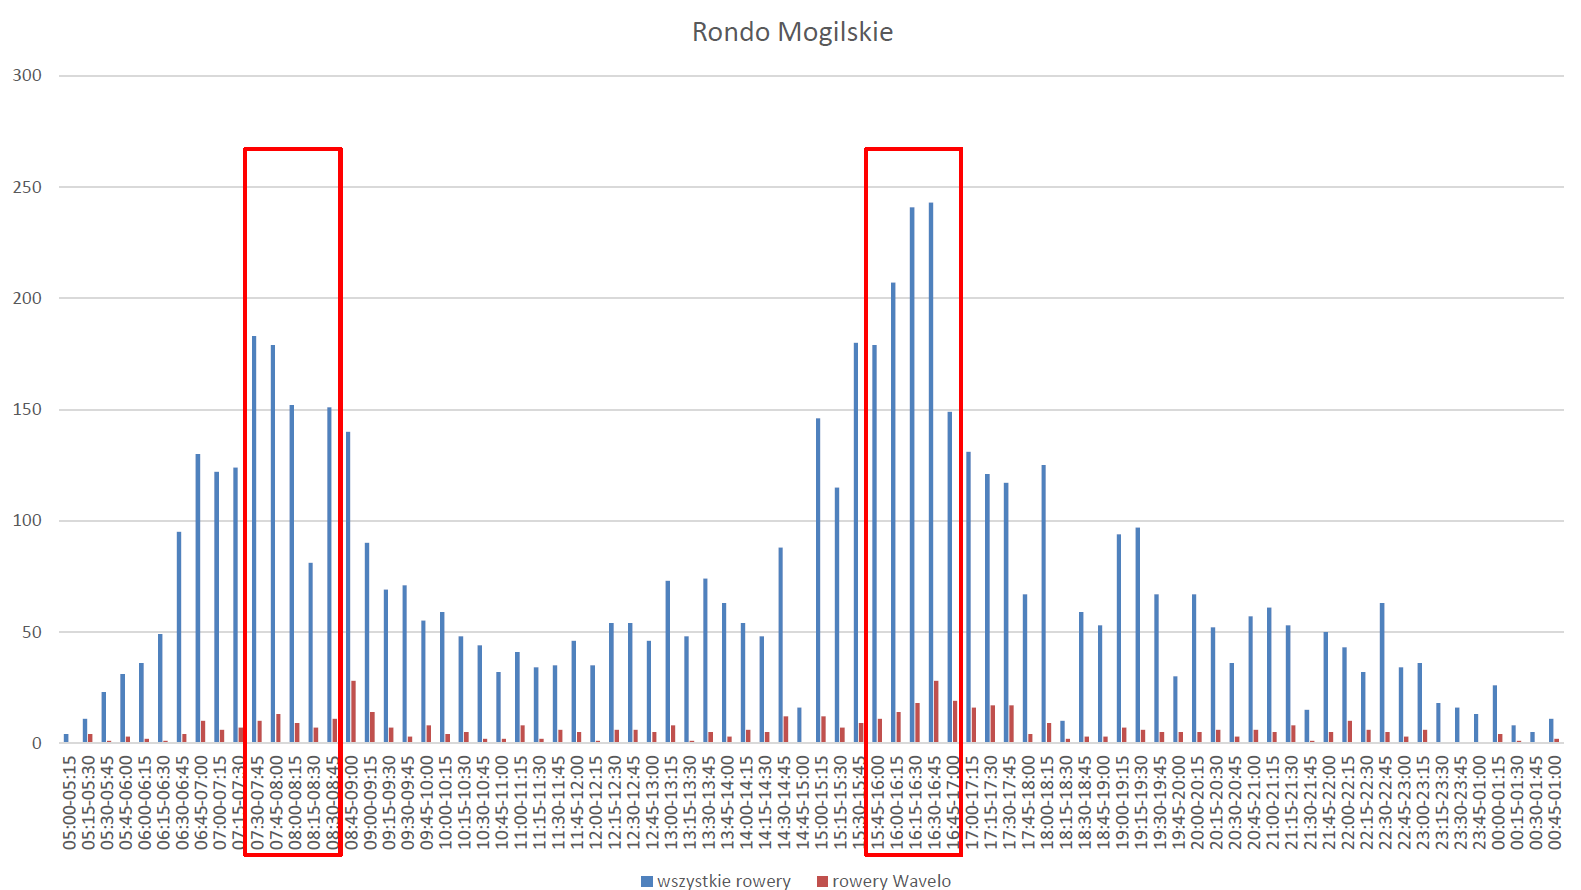
\includegraphics[width=\textwidth]{nat_ruchu_row}
\caption{[1]Natężenie ruchu rowerowego na Rondzie Mogilskim wg. Urzędu Miasta Krakowa (pomiar dokonany dnia 19.06.2018).}
\end{figure}
U podstaw niniejszego zjawiska leżą zróżnicowane przyczyny i nie wszystkie można wytłumaczyć powszechną modą na ekologię czy rosnącą popularnością roweru jako ogólnej formy rekreacji. Ważne aspekty, wpływające na wybór roweru jako środka komunikacji, to między innymi także takie kwestie jak możliwość bezproblemowego (w większości przypadków) dojazdu dokładnie do naszej destynacji, ekonomiczność takiego rodzaju komunikacji (jazda jest darmowa, jedynym wydatkiem jest kupno samego roweru), a w nierzadkich przypadkach i czasu (rower nie stoi w korkach, a jednocześnie jest dużo szybszy niż poruszanie się pieszo), czy korzyści zdrowotne wynikające z regularnego wysiłku fizycznego. Niemałym atutem roweru jest również jego łatwiejsze zaparkowanie – w centrach większych miast stojaki rowerowe są rozmieszczone całkiem gęsto i w zasadzie nigdy nie brakuje na nich miejsca, czego nie można powiedzieć o stanowiskach parkingowych dla samochodów. Te, oraz wiele innych przyczyn, pozwala zrozumieć dlaczego liczba amatorów bezsilnikowych jednośladów regularnie rośnie i nie wygląda na to by rosnąć miała przestać. Co istotniejsze nie tylko tych jeżdżących dla przyjemności w swoim czasie wolnym, ale także – a może przede wszystkim – tych korzystających z roweru jako zamiennika samochodu lub komunikacji zbiorowej. Tendencję tę można zauważyć zwłaszcza w miastach o bardzo dużym natężeniu ruchu samochodowego, co ułatwia wydedukowanie oczywistych zależności: w miastach odległości są względnie niewielkie, a powstające na głównych ciągach komunikacyjnych zatory w ruchu pojazdów mechanicznych, powodują znaczne wydłużenie czasu podróży przy użyciu tychże. Stąd rower całkiem często okazuje się wybawieniem, środkiem transportu, który zaoszczędza niemało czasu i niejako przy okazji daje okazję do poruszania się i spalenia palu kalorii. Dlatego też widok dużej ilości stojaków rowerowych ustawionych przy siedzibach największych firm nikogo nie dziwi. Wręcz przeciwnie – nie raz pracownicy jakiegoś przedsiębiorstwa potrafią wprost wypomnieć brak takiego udogodnienia.  
Obecna strategia każdego większego miasta – zwłaszcza europejskiego – opiera się niejako na stworzeniu jak największych możliwych udogodnień dla rowerzystów, jednocześnie starając się ograniczyć ruch samochodowy. Oba aspekty łączą się ze sobą w jedną spójną całość, a obrana przez miejskie władze ścieżka rozwoju nie jest podyktowana wyłącznie ekologią, ale także chłodną ekonomiczną kalkulacją. Metropolia, której drogi są permanentnie zakorkowane, w dłuższej (a czasem także i w krótszej) perspektywie czasu traci finansowo. Oczywiście straty te nie są bezpośrednie, a wynikają z odpływu mieszkańców, w efekcie czego spada liczba przedsiębiorstw, a koniec końców także i turystów.  Kraków nie chciał pozostać w tyle za innymi europejskimi miastami i również od kilku lat stara się inwestować w infrastrukturę rowerową, z gorszym lub lepszym skutkiem. Wprawdzie wdrażane i planowane inwestycje we wszelkiego rodzaju ścieżki rowerowe i innego typu udogodnienia nie zaspokajają znacznie szybciej rosnących potrzeb krakowskich rowerzystów, to jednak trzeba docenić fakt ich powstawania oraz zauważyć, że sieć tras już teraz jest całkiem przyzwoita. Efektem tego podróż z dowolnego miejsca w Krakowie przy pomocy bicykla nie jest już udręką i może być w dużej mierze realizowana po specjalnie wyznaczonym obszarze. Oczywiście lata zaniedbań powodują, że nie wszystko da się poprawić od razu, więc i w stolicy Małopolski nadal znajdują się białe plamy, gdzie teoretycznie dojazd rowerem umożliwia jedynie zwykła ulica, jednak takich miejsc systematycznie ubywa. Co najistotniejsze miejskie władze mocno skupiły się na tworzeniu ścieżek w najbardziej newralgicznych obszarach, dzięki czemu większość dużych skupisk ludzkich (gdzie na co dzień mieszka i sypia sporo mieszkańców) oraz dzielnic usługowo-handlowych czy też biznesowych (gdzie owi mieszkańcy pracują lub udają się na zakupy bądź relaks) jest ze sobą nad wyraz poprawnie skomunikowana pod względem rowerowym. \newline
Daje się jednak zauważyć, iż pomimo nie najgorszej infrastruktury, wielu krakowskich rowerzystów – często być może nieświadomie – nie wykorzystuje potencjału w niej drzemiącego. Widok rowerzysty poruszającego się po zwykłej drodze, podczas gdy istnieje alternatywna, wcale nie dłuższa ścieżka wytyczona specjalnie dla tego typu transportu, nie należy do rzadkości, pomimo faktu, iż rowerzysta ma obowiązek korzystania z drogi rowerowej, gdy ta jest poprowadzona bezpośrednio przy danej jezdni. A przecież taka sytuacja nie jest komfortowa ani dla użytkownika roweru, ani kierowcy samochodu, co więcej stanowi również dużo większe zagrożenie dla bezpieczeństwa rowerzysty. Niemałe jest także grono osób niezdecydowanych, dla których hasło „dojazd do pracy rowerem” lub podobne kojarzy się bardziej z koniecznością slalomu między samochodami, wdychaniem spalin i strachem przed potrąceniem, niż z oszczędnością czasu i pieniędzy. Tego typu ludzie również nie mają pełnej wiedzy na temat tego jak wygląda infrastruktura rowerowa w Krakowie, często przekonując się o tym dopiero po pierwszych przejazdach, metodą prób i błędów. Sytuacja ta wynika oczywiście ze sporej dynamiki rozwoju udogodnień dla rowerów, o której wspomniano wcześniej.
Trafnym staje się zatem pytanie: jak w łatwy sposób doinformować ludzi? Jak zachęcić ich do korzystania z rowerów? Rozwiązaniem wydaje się stworzenie czegoś w rodzaju swoistego przewodnika po infrastrukturze rowerowej Krakowa, dlaczego więc nie pójść krok dalej i nie stworzyć pełnoprawnej nawigacji rowerowej? Nie da się ukryć, że grupą społeczną, wśród której najprościej jest rozpropagować jakiś trend lub modę, jest grupa ludzi młodych, głównie przed 35 rokiem życia. W jaki sposób stworzyć u takich ludzi zainteresowanie? Oczywiście przy pomocy zawoalowania rozwiązania w kokon nowoczesnych rozwiązań, najlepiej więc by taka nawigacja była aplikacją na smartfony. To także poszerza dostępność rozwiązania, gdyż obecnie niemal każdy posiada smartfon. \newline
Nawigacja rowerowa w swym zamyśle ma więc nie tylko pomóc przeciętnemu rowerzyście w przemieszczaniu się po Krakowie, lecz także propagować taką formę transportu. Propagować i pomagać niezdecydowanym, tak by wybrali opcję rowerową. Wystarczy przecież rzut oka na wyznaczoną trasę pomiędzy interesującymi nas punktami i nagle okazuję się, że przejazd między nimi nie musi wiązać się z jazdą po ruchliwej ulicy. Niezwykle ważnym jest by aplikacja nie pozostała w tyle za szybkimi zmianami w topografii miasta, dlatego też musi być oparta o regularnie aktualizowane i niezawodne dane. Takimi bez wątpienia są dane tworzone przez instytucję, która ma bezpośredni wpływ na wygląd siatki ścieżek rowerowych w mieści, dlatego też aplikację opisaną w niniejszej pracy oparto na bazie danych ZTP.

\chapter{Testy}

\section{Test URL-a}

Wejdź na stronę \url{https://www.google.pl/} i wpisz szukane zdanie.

\clearpage

\section{Test dzielenia wdów}

Lorem ipsum dolor sit amet, ex est alia dolorem commune. Duo modo errem no. Ea harum doming atomorum mei. Consul animal malorum cu qui, sumo dicta graece an est, vim ei clita regione.

Vel eu quando doming fastidii, mei graeco indoctum an, legere theophrastus in pro. Te mei probatus eleifend interpretaris. Est no autem liber vituperatoribus, cu mea dicam constituto. Ea laudem tritani consectetuer sit, sanctus patrioque expetendis vix in. Duo id fugit adversarium signiferumque, an quot modus molestiae qui.

Ut paulo definiebas pro. Mea an quod esse. Et atomorum facilisis moderatius sit. Graeco iudicabit forensibus in vel. Eam cu lorem aeterno offendit, cu vix nulla congue posidonium. Vel lucilius evertitur vituperata no.

Mea eu graecis prodesset. Et tota eius nec. Ei etiam oratio has, vel ei homero eripuit invenire. Sed ex errem intellegebat, sea et elitr intellegat constituto. Nostro voluptua accusamus eos in, ei sale admodum has. Vim ne consetetur reformidans, ad has malis recusabo persequeris, per etiam virtute invenire in.

Te nihil eruditi eam, sit aperiam accusam mediocritatem at. Nec ne nonumy dictas disputationi, vis ridens sadipscing ex. Harum euripidis ex vix, at consetetur instructior signiferumque mel, at mei elitr honestatis. Id sit congue vituperata. Temporibus eloquentiam no eum.

Pro id esse phaedrum, nostro iudicabit eos ut. Sit ea aperiam alienum, harum audiam voluptua cu usu. Iudico invenire te vel, id suscipit disputando pri. Ut sumo expetenda mea.

Cum at idque nullam aperiam, vis ex aeque ponderum luptatum. Vix soluta graeco dissentiet ut, ut est reque periculis similique, ut dicta dicant repudiare sea. Ne dolor legendos signiferumque ius, at eirmod convenire qui. Suas numquam conceptam mei ex. Autem homero eos et, sea dicta alienum iudicabit ut.

Ea duo consulatu vulputate, id elit perpetua cum. His ei aeque saepe audiam. Prompta laoreet facilisi ne sed, per hinc consetetur te, oratio fuisset ullamcorper mel at. Quis suscipiantur ne nec, agam efficiendi usu in.

Vis eu iuvaret singulis appellantur, usu ex saepe omittantur. Sed possit mnesarchum at, usu illum choro oratio in, et debet dolor vix. Mel aperiri suscipiantur ne, te per illum fuisset, lorem pericula mei ad. Pri id tale lucilius dissentiet, id sea sonet expetenda. Agam sensibus persequeris sed no, eum at tamquam sanctus.

Omnis exerci soleat ut vis. Rebum vidisse sea ex. Ius animal gubergren efficiantur ad, mollis probatus nec ut. Meis platonem ex vel, ut qui tale tritani equidem. Vide meis fuisset mel at, nam an assum delenit gubergren. No illum reprimique vim, te augue nullam per, ludus dicant suscipiantur ne sed.

An pri mediocrem deseruisse, ad sumo audire dissentiet sit. Sit ea civibus lobortis. Etiam ceteros commune ei vis. Pro ei equidem vivendo. Quo ne prima periculis omittantur, ex rebum veritus sit, ei dolor maiestatis mea.

\subsection{Lorem ipsum}

Et mel munere quodsi sapientem. Essent legimus ne pro. Est ornatus definiebas et. No habemus docendi ius, purto sapientem mei at. Tamquam vivendo necessitatibus has at, no habemus praesent nec. No quo modus iudicabit scriptorem. Modus intellegebat ea vim. Cu ius lorem regione offendit, ne accusata sensibus vituperatoribus quo. Sit ut iuvaret indoctum. Ut mea sale justo. Sapientem definitionem ius eu, at sea quem doming. Facete conclusionemque ut nec, vix at duis eius. Eos quot consequuntur et, ornatus liberavisse ne mei.

Per an dicam commodo tractatos, usu in timeam numquam tacimates. Case delectus eu sea, usu audiam eleifend tincidunt id, nec at decore discere mentitum. Ut elit veri eloquentiam his, ceteros tractatos ea has. Duo impetus scribentur et, eu quo errem everti, ad recusabo consulatu ius. Fastidii comprehensam pri ea, ex duo augue quando denique. Eos aeterno deserunt sententiae cu, ius quas tation patrioque ex.

Id autem scripta explicari nec, congue quidam possit te sit. Et usu ipsum bonorum graecis, ferri verear deterruisset eum cu. Purto porro accommodare cu vim. Cum ei tritani pertinacia voluptaria.



% itd.
% \appendix
% \include{dodatekA}
% \include{dodatekB}
% itd.

\printbibliography

\end{document}
